% Graph 2
\documentclass[tikz]{standalone}
\usepackage{tikz}
\usetikzlibrary{bayesnet}

\begin{document}

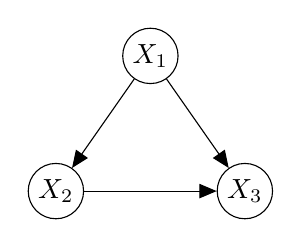
\begin{tikzpicture}
  % Nodes
  \node[latent] (X1) {$X_1$};
  \node[latent, below=of X1, xshift=-1.2cm] (X2) {$X_2$};
  \node[latent, below=of X1, xshift=1.2cm] (X3) {$X_3$};

  % Edges
  \edge {X1} {X2};
  \edge {X2} {X3};
  \edge {X1} {X3};
\end{tikzpicture}

\end{document}